\documentclass{beamer}
\usepackage{epstopdf}

\mode<presentation> {
	\usetheme{Malmoe}
	\usecolortheme{whale}
	\setbeamertemplate{footline}[page number]
	\setbeamertemplate{navigation symbols}{}
}

%----------------------------------------------------------------------------------------
%	TITLE PAGE
%----------------------------------------------------------------------------------------

\title[Short title]{Project NUClear}

\author{
	Trent Houliston \and Jake Woods \and Joshua Kearns \and Michael Burton
}

\institute[UoN]
{
	University of Newcastle \\ % Your institution for the title page
	\medskip
	\textit{Trent.Houliston@uon.edu.au, Jake.f.woods@gmail.com} % Email address
}

\date{\today}

% Start of document
\begin{document}

%----------------------------------------------------------------------------------------
% Title Slide 
%----------------------------------------------------------------------------------------
\begin{frame}
	\titlepage % Print the title page as the first slide
\end{frame}

%----------------------------------------------------------------------------------------
% Overview (Table of Contents)
%----------------------------------------------------------------------------------------
\begin{frame}
	\tableofcontents
\end{frame}

%----------------------------------------------------------------------------------------
\section{Introduction}
%----------------------------------------------------------------------------------------
\begin{frame}
\end{frame}

\begin{frame}
	\frametitle{Problem Description}
		Improve the software architecture of the NUbots robocup system to:
		\begin{itemize}
			\item Facilitate the use of robots for research, marketing, other non-soccer based behaviours.
			\item Improve the time it takes to become effective with the NUbots code.
			\item Make it easier to take full advantage of the robots hardware.
		\end{itemize}
\end{frame}

\begin{frame}
	\frametitle{Estimated Effort}
		Time \& Money
		\begin{itemize}
			\item 48 person-months of effort.
			\item Estimated cost of \$200,000 (using COCOMO)
		\end{itemize}
		
		Additional Factors
		\begin{itemize}
			\item Loss of team members
			\item Required a large set of companion documentation
		\end{itemize}
\end{frame}

%----------------------------------------------------------------------------------------
\section{Existing System}
%----------------------------------------------------------------------------------------
\begin{frame}
	\sectionpage
\end{frame}

\begin{frame}
	\frametitle{Existing System}
	\begin{itemize}
		\item The NUbots system has an existing system
	\end{itemize}
\end{frame}

%----------------------------------------------------------------------------------------
\section{New Design}
%----------------------------------------------------------------------------------------
\begin{frame}
	\sectionpage
\end{frame}

\begin{frame}
	\todo[inline]{Talk about coupling r.e. maintainablity}
	\todo[inline]{Diagram of different forms of coupling}
\end{frame}

\begin{frame}
	\todo[inline]{Describe message passing systems}
	\todo[inline]{How decoupled they are but they need a message passing management system}
\end{frame}

\begin{frame}
	\todo[inline]{Talk about existing systems such as Robot OS, DDX, CORBA}
\end{frame}

\begin{frame}
	\todo[inline]{These are all slow}
\end{frame}

\subsection{NUClear}
\begin{frame}
	\frametitle{NUClear}
	\begin{itemize}
		\item These systems are all too slow to use on a robot
		\item A new system must be designed if message passing is to be used
	\end{itemize}
\end{frame}

\begin{itemize}
	\item Problem description
	\item Number of lines of code, estimate of effort
	\item Good Software architecture
	\begin{itemize}
		\item Coupling
		\item Cohesion
	\end{itemize}
	\item Existing system
	\item ROS DDX etc message passing
	\item Metaprogramming
	\item NUClear API
	\begin{itemize}
		\item Message passing
		\item Networking
		\item Multithreading
	\end{itemize}
	\item Benefits
	\begin{itemize}
		\item 
	\end{itemize}
	\item Discuss the ease of adding in things
	\item Robot Dance
	\begin{itemize}
		\item What do they do?
		\item How does it work?
	\end{itemize}
	\item Demonstrate robot dancing
	\item Demonstrate live coding of auto getup script
	\item Demonstrate robot firing missiles
\end{itemize}




%----------------------------------------------------------------------------------------
\section{Robot Dance}
%----------------------------------------------------------------------------------------
	\subsection{What and Why?} %-------------------
	\begin{frame}
		\sectionpage %Title page for the Robot Dance section
	\end{frame}
	\begin{frame}
		\frametitle{Why make the robots dance?}
		\begin{itemize}
			\item How does this relate to the rest of the project?
			\begin{itemize}
				\item Demonstrates the efficiency of the new architecture
			\end{itemize}
			\item Why demonstrate the architecture through dancing robots?
			\begin{itemize}
				\item Tests the architecture in adding functionality unrelated to soccer
				\item Useful for marketing
			\end{itemize}
		\end{itemize}
	\end{frame}
	\begin{frame}
		\frametitle{How do they dance?}
		\begin{itemize}
			\item Originally we were going to make them dance in 3 ways:
			\begin{itemize}
				\item Scripted Dance Moves
				\item Dancing to music
				\item Copying human dance moves through the camera
			\end{itemize}
			\item Due to team members leaving:
			\begin{itemize}
				\item Unable to do dancing by copying human
			\end{itemize}
		\end{itemize}
	\end{frame}
	\subsection{Scripted Dance} %-------------------
	\begin{frame}
		\frametitle{Scripted Dance Moves}
		\begin{itemize}
			\item Most simple method of robot dance
			\item Dance script specifies:
			\begin{itemize}
				\item Angle for robot motors to move to
				\item Times for when the motors should get there
			\end{itemize}
			\item Can be used as part of dancing to music
			\item Can easily replace current soccer scripts
		\end{itemize}
	\end{frame}	
	\begin{frame}
		\frametitle{Creating the dance scripts}
	\end{frame}	
	\begin{frame}
		\frametitle{Dancing and the New Architecture}
		\framesubtitle{Dancing to a Script}
		\begin{figure}
			\centering
			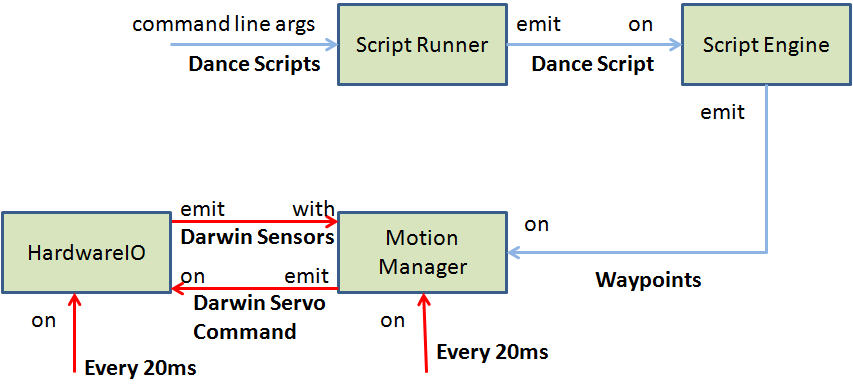
\includegraphics[scale=.5]{Presentation_Images/dance_script_new_arc.png}
			\caption{Components for Dancing to Script with Nuclear}
		\end{figure}
	\end{frame}	
	\begin{frame}
		\frametitle{Dancing and the New Architecture}
		\framesubtitle{Dancing to a Script}
		\begin{figure}
			\centering
			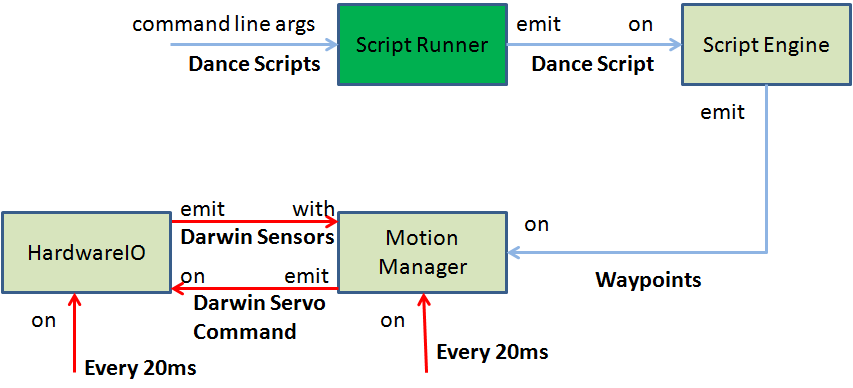
\includegraphics[scale=.5]{Presentation_Images/dance_script_new_arc_change.png}
			\caption{Components for Dancing to Script with Nuclear}
		\end{figure}
	\end{frame}
	\begin{frame}
		\frametitle{Dancing and the Old Architecture}
		\framesubtitle{Dancing to a Script}
		\begin{figure}
			\centering
			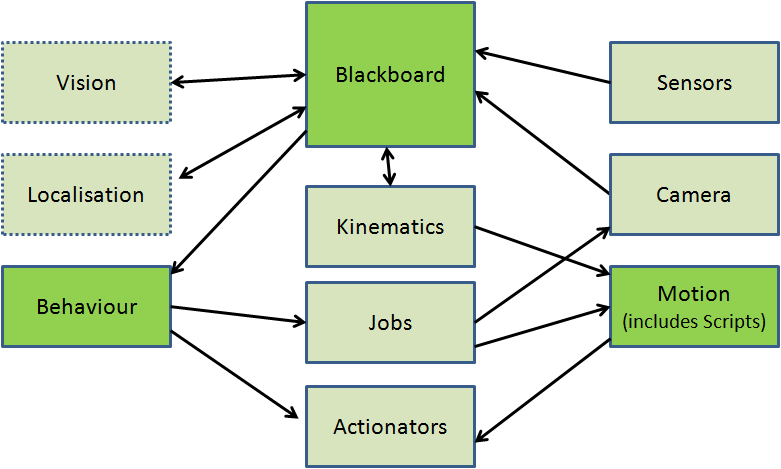
\includegraphics[scale=.45]{Presentation_Images/dance_script_old_arc.png}
			\caption{Components for Dancing to Script with the Old System}
		\end{figure}
	\end{frame}	
	\subsection{Dancing to Music} %-------------------
	\begin{frame}
		\frametitle{Dancing to Music}
		Things to consider:
		\begin{itemize}
			\item How to analyse music
			\begin{itemize}
				\item Holistic approach?
				\item Isolate musical characteristics?
			\end{itemize}
			\item Dance Moves
			\begin{itemize}
				\item Pre-Scripted or Dynamically Generated?
				\item Scope of movement. Involving legs or just upper body?
				\item How to relate dance moves to music
			\end{itemize}
		\end{itemize}
	\end{frame}	
	\begin{frame}
		\frametitle{Dancing to Music}
		\framesubtitle{Music Analysis}
		\begin{itemize}
			\item Beat is most important
			\item What is beat?
			\begin{itemize}
				\item Basic timing element of a song
				\item Tapping along to a song is finding the beat
			\end{itemize}
			\item Robot Dancing must be in time with beat
			\item Many other musical characteristics depend on beat
		\end{itemize}
	\end{frame}	
	\begin{frame}
		\frametitle{Dancing to Music}
		\framesubtitle{Finding the Beat}
		\begin{itemize}
			\item Finding the beat is known as Beat Tracking
			\item Beat Tracking must be:
			\begin{itemize}
				\item Real Time
				\item Predictive
				\item Quick
				\item Accurate
				\item Robust
			\end{itemize}
		\end{itemize}
	\end{frame}	
	\begin{frame}
		\frametitle{Dancing to Music}
		\framesubtitle{Beat and Dance}
		How we relate beat to dance:
		\begin{itemize}
			\item On Startup the dance Scripts are loaded
			\item When a beat is found, the Dance Engine is notified
			\item Each move in the dance script is reconfigured to be in time with the latest beat
			\item When no dance is currently being run, a new dance script is chosen to be run
		\end{itemize}
	\end{frame}	
	\begin{frame}
		\frametitle{Dancing and the New Architecture}
		\framesubtitle{Dancing to a Music}
		\begin{figure}
			\centering
			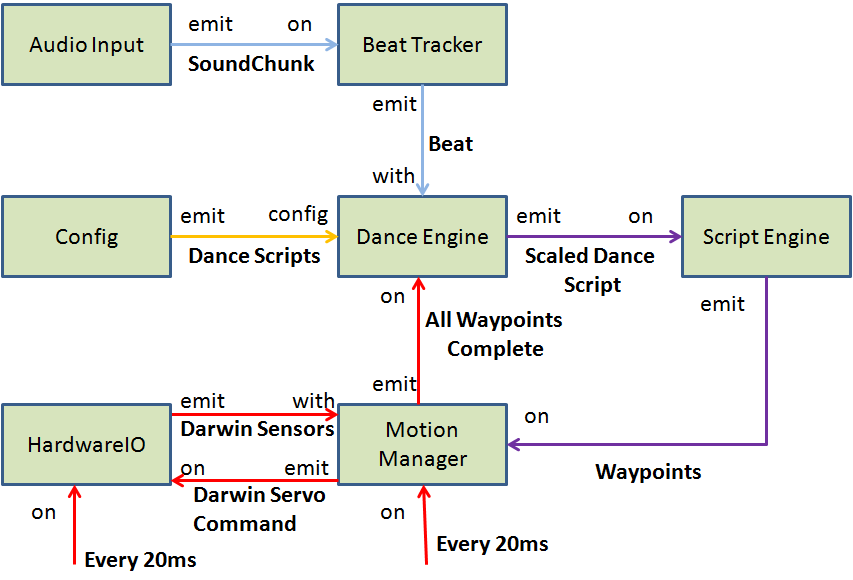
\includegraphics[scale=.45]{Presentation_Images/dance_audio_new_arc.png}
			\caption{Components for Dancing to Music with the NUClear}
		\end{figure}
	\end{frame}	
	\begin{frame}
		\frametitle{Dancing and the New Architecture}
		\framesubtitle{Dancing to a Music}
		\begin{figure}
			\centering
			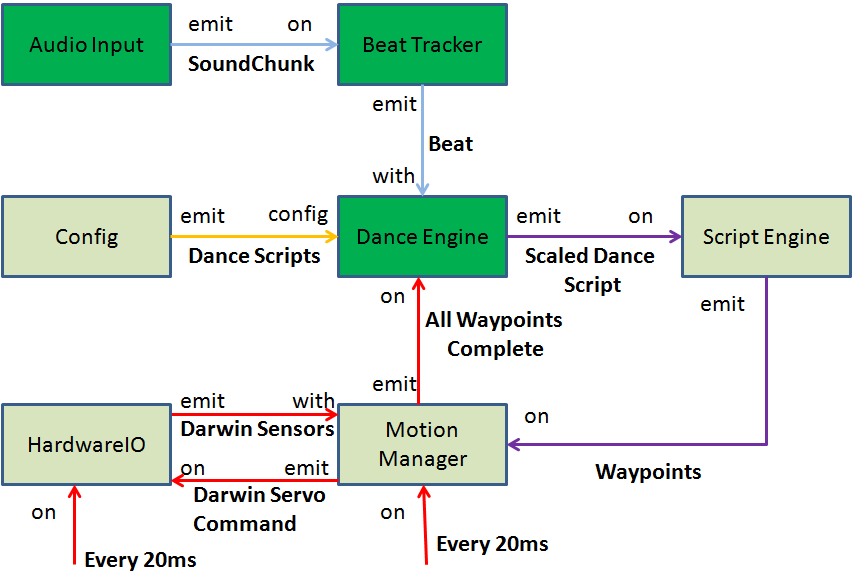
\includegraphics[scale=.45]{Presentation_Images/dance_audio_new_arc_change.png}
			\caption{Components for Dancing to Music with the NUClear}
		\end{figure}
	\end{frame}	
	\begin{frame}
		\frametitle{Dancing and the Old Architecture}
		\framesubtitle{Dancing to a Music}
		\begin{figure}
			\centering
			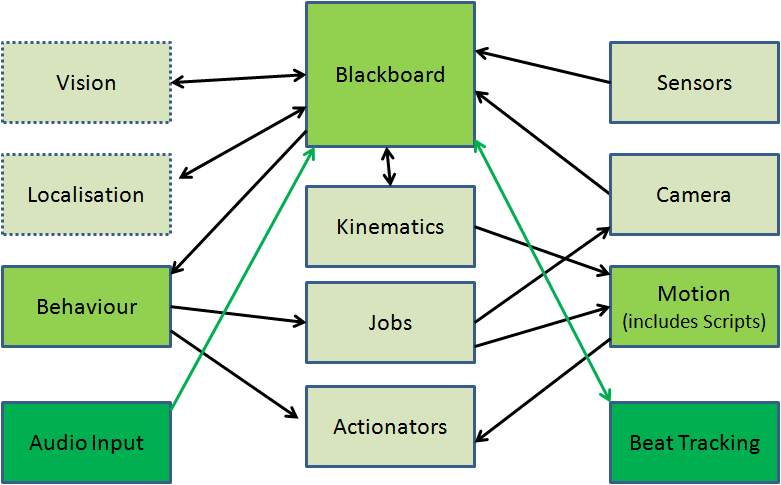
\includegraphics[scale=.45]{Presentation_Images/dance_audio_old_arc.png}
			\caption{Components for Dancing to Music with the Old System}
		\end{figure}
	\end{frame}	
	\subsection{Conclusions} %-------------------
	\begin{frame}
		\frametitle{Conclusions from Robot Dance}
			\begin{itemize}
				\item Robot Dance shows NUClear to be:
				\begin{itemize}
					\item Easy to learn
					\item Easy to use
					\item Modular
					\item Loosely Coupled
				\end{itemize}
			\end{itemize}
	\end{frame}	




%----------------------------------------------------------------------------------------
\section{Individual Research}
%----------------------------------------------------------------------------------------
\begin{frame}
	\sectionpage
\end{frame}

	%----------------------------------------------------------------------------------------
	\subsection{Overcoming Limits of Event Driven Systems}
	%----------------------------------------------------------------------------------------
	\begin{frame}
		\subsectionpage
	\end{frame}
	
	%----------------------------------------------------------------------------------------
	\subsection{Compile Time Message Routing}
	%----------------------------------------------------------------------------------------
	\begin{frame}
		\subsectionpage
	\end{frame}
	
	%----------------------------------------------------------------------------------------
	\subsection{Efficient Multithreading in Message Passing Systems}
	%----------------------------------------------------------------------------------------
	\begin{frame}
		\subsectionpage
	\end{frame}
	
	%----------------------------------------------------------------------------------------
	\subsection{Beat Detection}
	%----------------------------------------------------------------------------------------
	\begin{frame}
		\subsectionpage
	\end{frame}

\end{document} 
